\chapter[Validação dos Resultados]{Validação dos Resultados}

Nesse capítulo serão analisados os modelos propostos no capítulo anterior. Cada um dos modelos deverá selecionar um conjunto de características para ser utilizado em um classificador, e então deverão ter seus resultados coletados e comparados. 


\section{Validação dos Modelos}

Os modelos selecionados devem contribuir para um melhor desempenho de um dado modelo de Aprendizado de Máquina, sendo assim, serão testados utilizando uma base de dados e levando em consideração a acurácia do classificador. A base de dados a ser utilizada é a dos sobreviventes do titanic, e a MADELON, uma base utilizada para competições. Cada um dos modelos serão testados utilizando essas bases seguindo os seguintes critérios:

\begin{enumerate}
	\item{Será utilizado o classificador kNN (\textit{k-Nearest Neighbours})}
	\item{Será realizado um pré-processamento na base de dados para:}
		\subitem{Remover características que sejam do tipo texto}
		\subitem{Substituir os campos vazios pela mediana daquele campo}
	\item{Da base de dados, será utilizado 2/3 dela para realizar o treinamento e 1/3 para realizar os testes}
	\item{Cada modelo deverá ser executado 10 vezes e o desempenho final será a média desses resultados.}
\end{enumerate}

O classificador escolhido foi o \textit{k-Nearest Neighbours} por ser um classificador simples apesar de ser computacionalmente exaustivo. Um dos motivos que levaram a escolha desse classificador é o fato de que ele é muito sensível às características irrelevantes, fazendo com que o processo de seleção de características seja um forte aliado a esse classificador.

Para cada uma das bases será realizada o procedimento apontado no diagrama da Figura 11.

\begin{figure}[H]
	\centering
	\label{fig10}
		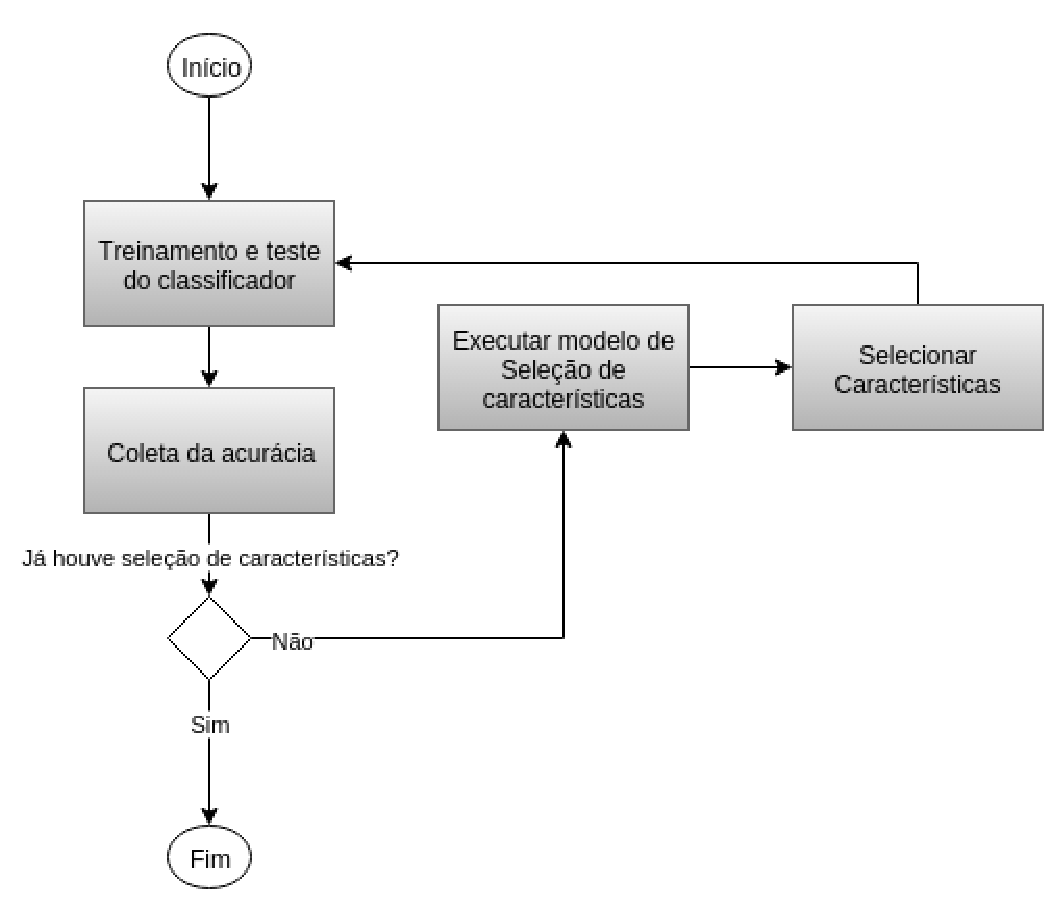
\includegraphics[keepaspectratio=true,scale=0.6]{figuras/fig10.eps}
	\caption{Fluxograma da validação dos resultados}
\end{figure}

\begin{enumerate}
	\item{Treinamento do classificador com 2/3 da base de dados sem nenhum processo de seleção}
	\item{Coleta da acurácia obtida do classificador após serem feitos os testes com 1/3 da base}
	\item{Realização do processo de seleção de características} 
	\item{Treinamento do classificador utilizando somente as características selecionadas}
	\item{Coleta da acurácia obtida do classificador após serem feitos os processos de seleção e os testes com 1/3 da base}
\end{enumerate}


As características da base de dados do Titanic, após ser realizado o pré processamento, se encontram da seguinte maneira descrito na Tabela 1.

\begin{table}[H]
\centering
\caption{Características da base Titanic}
\label{my-label}
\begin{tabular}{|l|l|}
\hline
\textbf{Característica} & \textbf{Tipo}            \\ \hline
survived                & Nominal \{0, 1\}         \\ \hline
pClass                  & Numérico                 \\ \hline
sex                     & Nominal \{male, female\} \\ \hline
age                     & Numérico                 \\ \hline
sibsp                   & Numérico                 \\ \hline
parch                   & Numérico                 \\ \hline
fare                    & Numérico                 \\ \hline
embarked                & Nominal \{Q,S,C\}        \\ \hline
\end{tabular}
\end{table}

O classificador a ser utilizado, as instancias e a acurácia inicial do classificador se encontram descritos na Tabela 2.

\begin{table}[H]
\centering
\caption{Informações sobre o classificador e instancias da base Titanic}
\label{my-label}
\begin{tabular}{|l|l|}
\hline
\textbf{Classificador}        & \multicolumn{1}{c|}{\textbf{kNN (Weka.IBk)}} \\ \hline
N. de características inicial & 8                                            \\ \hline
Acurácia inicial média        & 72.8977\%                                   \\ \hline
Instancias para treino        & 607                                          \\ \hline
Instancias para teste         & 303                                           \\ \hline
\end{tabular}
\end{table}

Após cada um dos métodos de seleção serem aplicados à base de dados, os resultados obtidos estão expostos na Tabela 3:

\begin{table}[H]
\centering
\caption{Resultados dos modelos - base Titanic}
\label{my-label}
\begin{tabular}{|c|c|c|}
\hline
\multicolumn{1}{|l|}{\textbf{Modelo}} & \textbf{Características Mantidas} & \multicolumn{1}{l|}{\textbf{Acurácia média Classificador}} \\ \hline
Relief-F                              & sex, pClass, age                  & 80.5281\%                                            \\ \hline
DTM                                   & sex, age, sibsp, pclass, fare     & 78.5479\%                                            \\ \hline
LFS                                   & sex, fare                         & 81.538\%                                             \\ \hline
\end{tabular}
\end{table}

Pode-se verificar que o processo de seleção de características foi efetivo, uma vez que ele diminuiu o número de características utilizadas inicialmente, além de aumentar a acurácia do classificador. Não foi feita qualquer alteração no classificador, a única mudança foi no número de características utilizadas.

Os resultados acima são para uma base com poucas características mas ainda sim foi possível ver uma melhora no desempenho do classificador. A base do Titanic é executada em poucos segundos, sendo impossível verificar o fato de que a diminuição de características leva a um melhor desempenho no quesito computacional. Para poder melhor exemplificar esse atributo será utilizado uma base maior. 

\citeonline{madelon_2003} é uma base de dados artificial que foi parte de um desafio chamado NIPS, realizado em 2003. É um problema de duas classes que tem como característica ser altamente não linear. A base de dados consta com 1820 instancias e 500 características, alem da classe. Mantendo o planejamento inicial, que é de utilizar 1/3 da base para realizar os testes, temos o status inicial do classificador da seguinte maneira:

\begin{table}[H]
\centering
\caption{Informações sobre o classificador e instancias da base MADELON}
\label{my-label}
\begin{tabular}{|l|l|}
\hline
\textbf{Classificador}        & \multicolumn{1}{c|}{\textbf{KNN (Weka.IBk)}} \\ \hline
Base de dados                 & MADELON                               \\ \hline
N. de características inicial & 500                                        \\ \hline
Acurácia inicial média        & 52.0194\%                                   \\ \hline
Tempo para treinamento        & 12 segundos                                  \\ \hline
Instancias para treino        & 1227                                          \\ \hline
Instancias para teste         & 613                                          \\ \hline
\end{tabular}
\end{table}


Após cada um dos métodos de seleção ser aplicado à base de dados, os resultados obtidos estão expostos na Tabela 5:

\begin{table}[H]
\centering
\caption{Resultados dos modelos - base MADELON}
\label{my-label}
\begin{tabular}{|c|c|c|c|c|}
\hline
\textbf{Modelo} & \textbf{\begin{tabular}[c]{@{}c@{}}Características \\ Mantidas\end{tabular}}                                                                                                                                           & \textbf{\begin{tabular}[c]{@{}c@{}}Acurácia \\ média do \\ Classificador\end{tabular}} & \textbf{\begin{tabular}[c]{@{}c@{}}Tempo de\\ treinamento \\ médio\end{tabular}} & \textbf{\begin{tabular}[c]{@{}c@{}}Tempo medio \\ para selecionar \\ características\end{tabular}} \\ \hline
Relief-F        & \begin{tabular}[c]{@{}c@{}}a\_28, a\_48, a\_64, \\ a\_105, a\_128, a\_153, \\ a\_241, a\_281, a\_318, \\ a\_336, a\_338, a\_378, \\ a\_433, a\_442, a\_451, \\ a\_453, a\_455, a\_472, \\ a\_475, a\_493.\end{tabular} & 88.6914\%                                                                  & \textless 1 segundo                                                     & 37 segundos                                                                                  \\ \hline
DTM             & \begin{tabular}[c]{@{}c@{}}a\_105, a\_442, a\_338, \\ a\_475, a\_451, a\_128, \\ a\_28, a\_336, a\_119, \\ a\_493, a\_48, a\_251, \\ a\_292, a\_318, a\_433\end{tabular}                                               & 80.937\%                                                                   & \textless 1 segundo                                                     & 2 segundos                                                                                   \\ \hline
LFS             & \begin{tabular}[c]{@{}c@{}}a\_105, a\_128, a\_241, \\ a\_336, a\_338, a\_442\end{tabular}                                                                                                                              & 91.2601\%                                                                  & \textless 1 segundo.                                                    & 332 segundos                                                                                 \\ \hline
\end{tabular}
\end{table}

Como é possível observar, o número de características selecionado foi menor do que 10\% do número inicial e o desempenho do classificador foi aumentado em até 40\%. O tempo gasto para realizar seu treinamento foi diminuído drásticamente, houve um gasto de tempo para realizar a seleção, porém os ganhos obtidos em questão de performance computacional e performance da acurácia de seleção mostram que o processo de seleção proporcionou melhorias de grande peso.
